\subsection{Конфигурация на микроконтролера}

\subsubsection{Стартиране }

Написан е прост стартиращ скрипт на ARM assembly за целите на проекта, който инициализира SP на процесора и инициализира PC=Resethandler.
Скриптът дефинира символите от таблицата за прекъсванията, като .weak референции, към DefaultHandler, който изпълнява безкраен празен цикъл.
Този скрипт има за цел да инициализира .bss секцията на контролера,
както и всички статични променливи, като използва позициите, генерирани от линкерния скрипт, както и да извика функцията за системна инициализация, след което се извиква main финкцията.

\subsubsection{Системна инициализация}

В тази фаза се налага да бъде инициализиран системният часовник.
В нашия случай ще инициализираме системния часовник от високочестотния външен осцилатор (HSE). 
Тъй като при стартиране се използва високочестотният вътрешен осцилатор (HSI), който е
неточен и може да доведе до синхронизационни проблеми при асинхронни комуникации 
с висок baud-rate като UART.
Поради тази причина се налага инициализирането на системния часовник с времева основа
високочестотния външен осцилатор (HSE), тъй-като е много по прецизен.
Високочестотният външен осцилатор (HSE) на платката е с честота 8MHz, затова използваме
хардуерния PLL модул за увеличаване на честотата със следните настройки:
\begin{verbatim}
    (PLL_M=8, PLL_N=336, PLL_P=2, PLL_Q=7)
\end{verbatim}
, като така получаваме  168MHz честота на системния часовник.
След това инициализираме делителите на честота за отделните шини:
\begin{verbatim}
    (AHB_Prescaler=1, APB1_Prescaler=4, APB2_Prescaler=2).
\end{verbatim}
След настройката на часовниците получаваме следните честоти за отделните шини (\autoref{fig:frequencies})

\begin{figure}[htpb!]
    \centering
    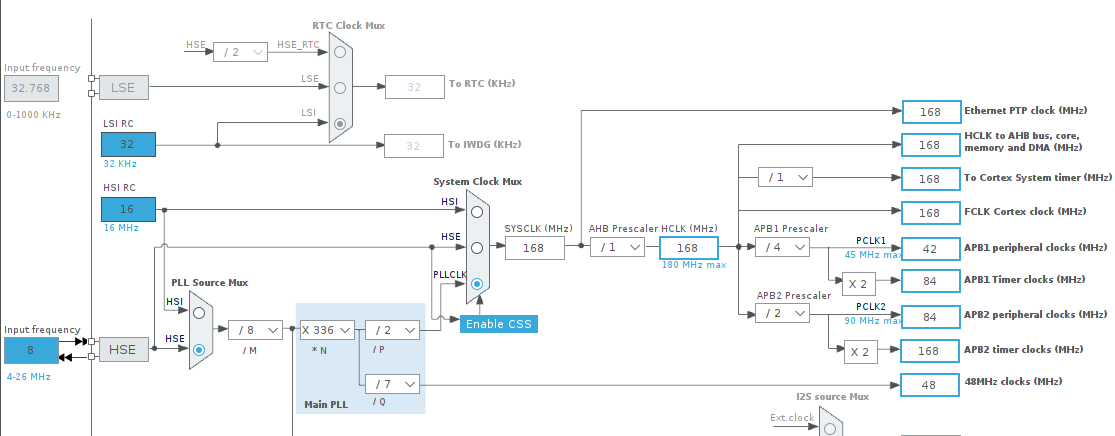
\includegraphics[width=0.9\textwidth]{frequencies}
    \caption{Честоти на системните шини и часовници след конфигурация}
    \label{fig:frequencies}
\end{figure}

Дуга основна част на системанта инициализация е инициализирането на хардуерния модул за числа с плаваща запетая (FPU).
Тъй като от конфигурацията (\autoref{lst:make_config}) настройваме комилатора за работа с модула за числа с плаваща запетая, е важно
преди която и да е операция с числа с плаваща запетая този модул да бъде инициализиран.
Необходимо е инициализацията на FPU да се случи преди преминването в ограничен режим.
Инициализацията се случва чрез блока от код (\autoref{lst:enable_fpu}).
\begin{lstlisting}[language=c, caption={Инициализация на модула за числа с плаваща запетая}, label={lst:enable_fpu}]
    /* Enable The FPU*/
    uint32_t* CPACR = (uint32_t*)0xE000ED88;
    *CPACR |=  0b00000000111100000000000000000000;
\end{lstlisting}

\subsubsection{Инициализация на периферията}

В тази фаза се инициализират периферните устройства като таймери, драйвъри за комуникационни протоколи и т.н.
Важно е да се отбележи, че преди инициализирането на който и да е периферен драйвър е нужно неговият часовник да бъде разрашен,
като се използва rcc интерфейса за шината, на която е закачен.

\paragraph{USART}:

Инициализиран е USART1, 
който се използва за извеждане на информация от 
конторлера и получаване на команди.
USART1 e инициализиран с конфигурация -- 
baud-rate 115200; 
дължина на думата 8 бита;
брой стоп битове 1;
Режим приемник/предавател.

За вход и изход на модула са инициализирани пинове PB6 и PB7.

За обработка на постъпващите команди е разрешено прекъсване (USART1\_IRQHandler),
което обработва прекъсванията, свързани с получаване на команди.

За целите на обработка на команди е съставен прост краен автомат, който 
да обработва постъпващите команди.
За момента командният интерфейс поддържа команди за задаване на
управляващо въздействие на избран канал, управляващ ESC.

\paragraph{I2C:}

Инициализиран е I2C3,
който се използва за комуникация със сензорите (жироскоп, акселерометър).
Използвана е следната конфигурация --
честота на I2C часовник 100000 Hz;
Режим I2C;
Адресиране 7 бита;

Поради факта, че периферните устройства, използващи I2C 
изискват запазване на състояние, което не можде изцяло да 
бъде възстановено от регистрите на I2C периферията,
е съставен краен автомат, който да управлява четенето и 
писането на блок от адреси само през прекъсването.
Така избягваме нуждата да изчакваме комуникацията да завърши
всеки отделен стадий и се използва прекъсването в комбинация
с краен автомат, който използваме за вземане на решенията.

Тъй-като връзката (хардуерно) не е високо надеждна
(jumper кабели), се случва периферията да се окаже в
състояние на грешка поради загуба на арбитрация или
друг тип грешка.
Пpоблемът е решен чрез използването на (I2C3\_ER\_IRQHandler),
като при възникване на проблем рестартираме или реинициализираме
периферията, за да продължим комуникацията.

\paragraph{Таймери:}

Инициализирани са таймери TIM2, TIM3, TIM5 и TIM7. 

TIM2 е с период 50Hz и се използва в режим Output-compare.
Този таймер генерира сигналите за упраление и има резолюция \(1\mu s\).

TIM3 и TIM5 са кофигурирани с резолюция \(0.2\mu s\) и се използват за приемане на сигналите, подадени от оператора през приемника.

TIM10 е конфигуриран с честота 52Hz, като се използва за прочитане на сензорите и обработка на получените сурови данни.


